\PageHeading{03}{产品流程与人机协作}{操作者是销售员，目标人群是销售员面前的客户}
\begin{tabularx}{\linewidth}{P{10mm}P{31mm}Y}
\rowcolor{Forest}\color{white}\bfseries 步骤 & \color{white}\bfseries 用户操作 & \color{white}\bfseries 系统反馈与约束\\
01 & 欢迎与接入 & 查看程序介绍、配置模型/ima连接并验证；密钥保留在服务端内存。\\
02 & 锁定产品 & 选择具体型号和系统版本，建立事实及图片归属边界。\\
03 & 明确客户与场景 & 选择8类场景或自定义；记录人群、目标和购买阶段，不静默覆盖客户。\\
04 & 选择渠道 & 从四渠道中选择所需渠道，分别形成结构、语气与配图策略。\\
05 & 补充要求 & 可输入自由提示词；无法确认的产品能力仍受证据约束。\\
06 & 共创并确认大纲 & 编辑标题、导语、段落、引用及配图；保存/AI修改产生新版本。\\
07 & 正文与视觉成品 & 展示SSE进度、事实依据和审核结果；预览、复制、单文件/ZIP导出。\\
\bottomrule
\end{tabularx}
\vspace{4mm}
\begin{minipage}[t]{.46\linewidth}
\Sub{大纲是明确的协作边界}
销售员先决定“写什么、按什么顺序写、用哪些依据与图片”。后端确认版本后复制快照；写作模型只能展开文本，不能改写已确认标题、段落结构、引用和图片集合。

\Lead{编辑体验}\par
未保存内容不能确认或生成；AI修改与手动保存均取消旧确认。取消长任务保留已保存大纲和上次正文，版本冲突提示重新载入，避免把旧稿误当成本次结果。

\begin{note}\small
更改产品、人群、场景或渠道后重新建立大纲。切换成品模板只重新排版，不能借此绕过事实审核。
\end{note}
\end{minipage}\hfill
\begin{minipage}[t]{.49\linewidth}
\vspace{0pt}\centering
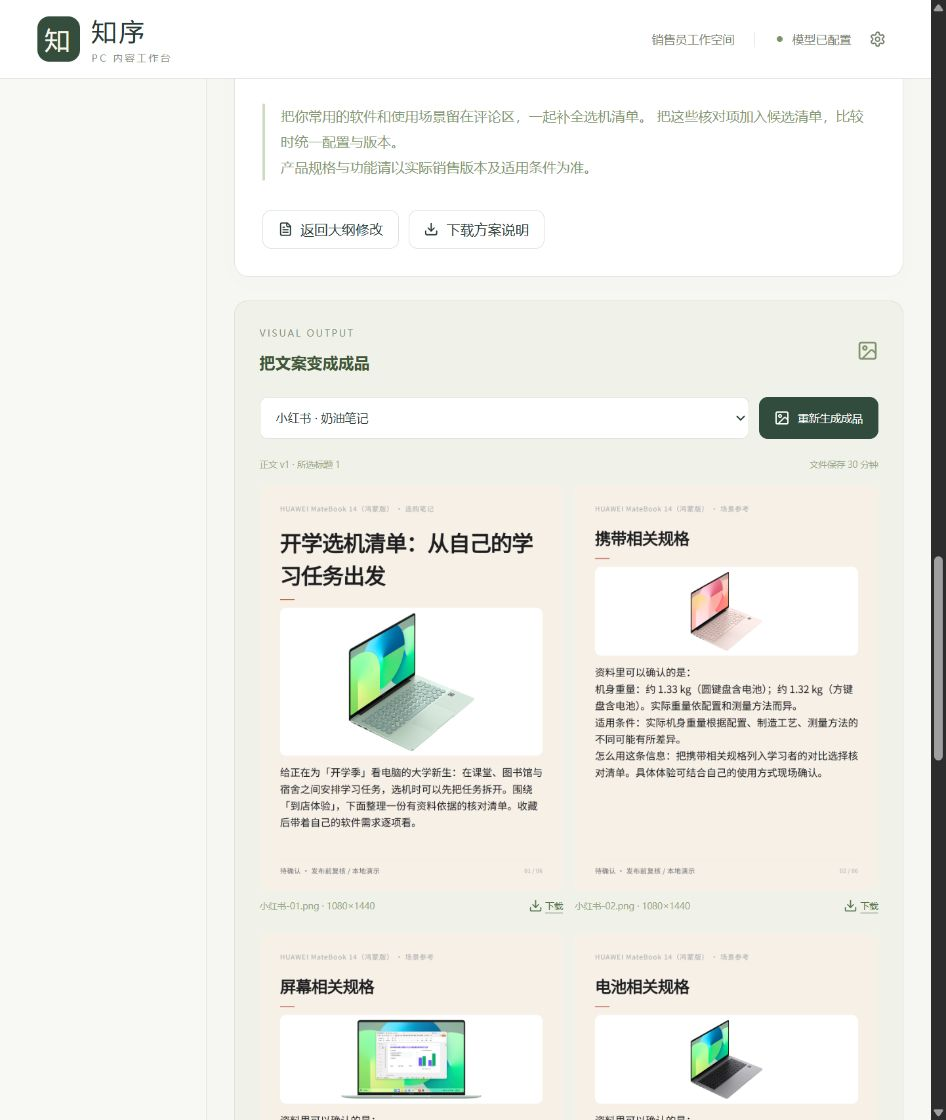
\includegraphics[width=\linewidth,height=107mm,keepaspectratio]{workflow-result.png}
\ImgCap{已保存的实际工作台截图：正文、返回大纲、模板选择和多页成品预览。此图来自本地演示，不表示ima验收。}
\end{minipage}
\SourceNote{前端WorkflowApp、RenderPanel，后端outlines与generate-from-outline；历史浏览器验收记录。}
